\subsection{Database Design}\label{InitialDesign}

In section \ref{currentState}, we outlined how the code from last year was left in an unfinished and undocumented state. Because of this, we estimated that starting over would give more value to the pipeline rather than spending time trying to understand and document it.

As mentioned in section \ref{ORM}, we opted to use EF Core to communicate with the database from the C\# application.

Despite the many advantages of this approach, it resulted in a database design that had major space issue.
In our rush to quickly implement the redesign, we unfortunately overlooked how to effectively store words from articles. 

Currently, we just store every single word in the database without regard for duplicates, which takes up way more space than necessary. Thus, it is not of the third normal form, and therefore not in BCNF either.
Ideally, we should instead store each word only once with an associated counter for how many times the given appears in an article.
We realize the issues with the current design and would like to address them in the near-future if time permits it.

The current database design is captured in the ER-diagram in figure \ref{newdatabaseER}.

\begin{figure}[htb!]
    \centering
    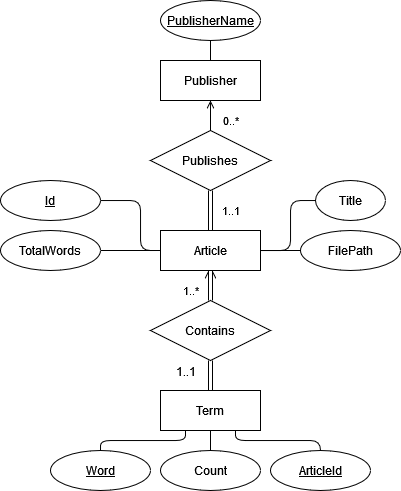
\includegraphics[scale=0.6]{Images/DbRedesign.png}
    \caption{ER diagram of the new database model.}
    \label{newdatabaseER}
\end{figure}

%\vspace{2cm}